\section{Experiment Setup}\label{sec:4}

\paragraph{Datasets.} Text: WikiText-103~\cite{ref19}, 200,000 contiguous samples (min.\ 512-character length) tokenized with GPT-2 BPE~\cite{ref4}, total $\approx$103M tokens. Vision: MS-COCO captions (2017 val split)~\cite{ref20}, 5,000 images / 25,000 captions, $224 \times 224$ ImageNet-normalized. Audio: LibriSpeech train-clean-100~\cite{ref21}, 10,000 indexed utterances at 16\,kHz / 80-mel. World: 20,000 episodes from \texttt{MiniGrid-Empty-8x8-v0}~\cite{ref22}, recording $(\mathrm{frame}_t, a_t, \mathrm{frame}_{t+1})$ triples with six discrete actions.

\paragraph{Model scales.} Three configurations with hard-capped total parameter budget (Table~\ref{tab:2}, Fig.~\ref{fig:3}). Compass rank $r = H/8$. All three fit within 6\,GB VRAM at 1024-token context.

\begin{table}[H]
\centering
\small
\begin{tabular}{lcccccccccc}
\toprule
Scale & $H$ & $L_{\mathrm{LM}}$ & $L_{\mathrm{WM}}$ & $r$ & LM core & Vision & Audio & World & Total & W/LM \\
\midrule
60m  & 384 & 10 & 10 & 48 & 33.4M  & 4.6M & 4.7M & 15.0M & \textbf{57.7M}  & 45\% \\
120m & 640 & 11 & 9  & 80 & 74.6M  & 4.7M & 4.8M & 37.6M & \textbf{121.7M} & 50\% \\
180m & 768 & 14 & 9  & 96 & 115.9M & 4.7M & 4.8M & 54.0M & \textbf{179.4M} & 47\% \\
\bottomrule
\end{tabular}
\caption{Three model configurations with verified parameter counts. $L_{\mathrm{LM}}$ is LM-block depth; $L_{\mathrm{WM}}$ is world-model TransitionModel depth.}
\label{tab:2}
\end{table}

\paragraph{Training protocol.} Each scale is trained for 10,000 optimizer steps ($\approx$650M tokens observed per scale). Training runs sequentially on the same physical GPU in the order 60m $\rightarrow$ 120m $\rightarrow$ 180m. Checkpoints saved every 2,000 steps. All experiments are reproducible from \texttt{python3 download\_poc\_data.py} followed by \texttt{python3 train\_quatrix\_poc.py --all --steps 10000} plus the three text-only variants.

\begin{figure}[H]
\centering
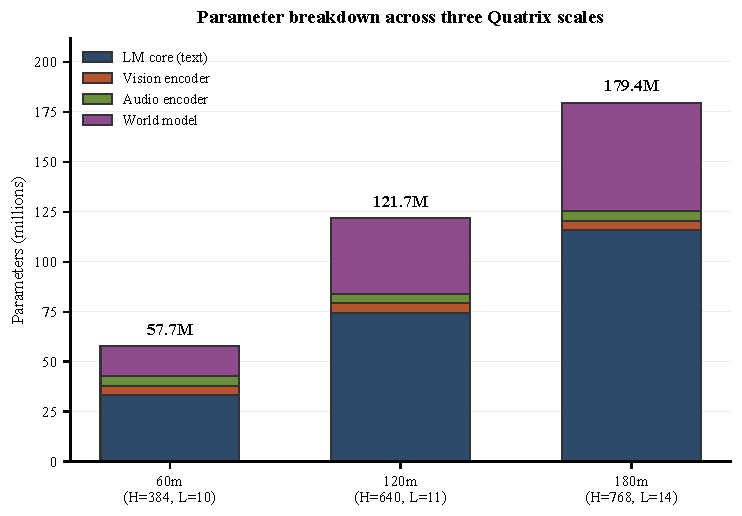
\includegraphics[width=.789\linewidth]{figs/fig03.pdf}
\caption{\textbf{Parameter breakdown across three \textsc{Quatrix} scales.} LM core grows from 33M to 116M as $H$ and $L_{\mathrm{LM}}$ increase; the world model is sized to $\sim$50\% of the LM core at each scale. Vision and audio encoders retain fixed internal sizes (384-hidden, 3 bidirectional layers each).}
\label{fig:3}
\end{figure}

\paragraph{Hardware.} A single NVIDIA RTX 4050 laptop GPU (6\,GB VRAM). Total wall-clock for the complete 3-scale sweep is approximately 24--36 hours.

\section{Results}\label{sec:5}

We report text-only and multimodal scaling at three parameter scales, plus held-out OOD evaluation on arxiv + pubmed.

\subsection{60m convergence on all four modalities}\label{sec:5.1}

\textsc{Quatrix}-60m (57.7M parameters) trains stably on the 4-modality mixture for 10,000 optimizer steps with no numerical issues (Fig.~\ref{fig:4}). All four per-modality training losses decrease through the full budget; the same stable training behaviour is observed at 120m and 180m.

\begin{figure}[H]
\centering
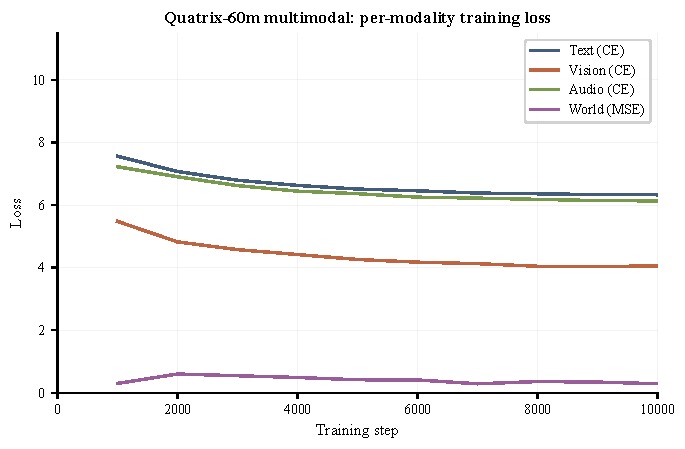
\includegraphics[width=.729\linewidth]{figs/fig04.pdf}
\caption{\textbf{\textsc{Quatrix}-60m multimodal training loss (10,000 steps).} Per-modality training cross-entropy (text/vision/audio) and world-model MSE on the unified 4-modality run. Mixture ratio 35/25/20/20. World-MSE drops from 1.125 at initialisation to 0.287 at step 10,000 in encoded-state space (the StateEncoder is trained jointly with the TransitionModel; the predict-mean baseline on the same encoder is reported in \S\ref{sec:6.3}).}
\label{fig:4}
\end{figure}

\paragraph{Per-modality held-out evaluation across three scales.} Held-out splits: WikiText-103 val (text, 1,038 docs), MS-COCO captions 5\% tail (vision, 1,250 docs), LibriSpeech 5\% tail (audio, 500 utterances), MiniGrid 5\% tail (world, 1,000 triples).

\begin{table}[H]
\centering
\small
\resizebox{\linewidth}{!}{%
\begin{tabular}{lrrrr}
\toprule
Modality / loss & 60m SAO MM & 120m SAVO MM & 180m SAVO MM & Best \\
\midrule
Text (CE, nats $\rightarrow$ ppl)   & $6.238 \rightarrow 512$ & $6.064 \rightarrow \mathbf{430}$ & $6.119 \rightarrow 454$ & 120m \\
Vision (CE, nats $\rightarrow$ ppl) & $5.166 \rightarrow 175$ & $4.870 \rightarrow 130$ & $4.858 \rightarrow \mathbf{129}$ & 180m \\
Audio (CE, nats $\rightarrow$ ppl)  & $7.552 \rightarrow \mathbf{1{,}905}$ & $7.582 \rightarrow 1{,}962$ & $7.610 \rightarrow 2{,}018$ & 60m \\
World (MSE) & 0.406 & 0.407 & 0.071 & 180m raw; predict-mean 0.033 \\
\bottomrule
\end{tabular}}
\caption{\textbf{Multimodal per-modality held-out evaluation.} Different modalities show different scaling regimes at the 10,000-step training budget: vision improves monotonically; text regresses 120m$\rightarrow$180m in lock-step with the text-only regression (\S\ref{sec:5.6}); audio is in a saturated band. World MSE drops 5.7$\times$ from 60m to 180m in encoded-state space; the predict-mean baseline on the trained 180m StateEncoder sits in the same band (0.033 vs trained 0.071), reflecting MiniGrid-Empty-8x8's low next-state variance (\S\ref{sec:6.3}).}
\label{tab:3}
\end{table}

\begin{figure}[H]
\centering
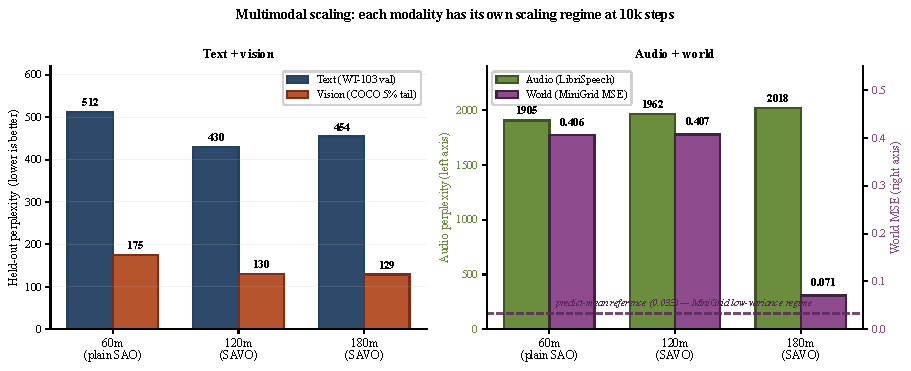
\includegraphics[width=.969\linewidth]{figs/fig05.pdf}
\caption{\textbf{Multimodal scaling per modality across 60m / 120m / 180m.} Left: text and vision held-out perplexity. Vision is monotonic; text peaks at 120m and regresses at 180m, in lock-step with the text-only regression at the same scales. Right: audio (left axis) and world MSE (right axis). World MSE drops from $\sim$0.41 at 60m/120m to 0.071 at 180m; the predict-mean reference line at 0.033 (computed on the trained 180m StateEncoder) is in the same band, reflecting MiniGrid's low encoded-state variance (\S\ref{sec:6.3}).}
\label{fig:5}
\end{figure}

\subsection{60m text-LM head-to-head: \QC{} vs.\ rank-matched attention}\label{sec:5.2}

To isolate the effect of the \QC{} primitive, we train a matched-architecture transformer baseline at 60m: same hidden size, layer count, FFN ratio, optimizer, data, and training budget, but with standard multi-head attention instead of \QC{}. All three attention projections ($W_Q, W_K, W_V$) are at rank $r = 48$, matching \QC{}'s $W_s, W_a$ rank, so the only architectural difference is whether content is gathered through a learned value projection $W_V$ (transformer) or directly from $x$ (\QC{}). This is a controlled ablation isolating the value-projection question, not a comparison against full-rank standard multi-head attention; a real-world Transformer-base baseline at full QKV rank (or with GQA / MQA at standard configurations) is left to future work, and the absolute perplexity numbers in this paper (val ppl $\sim$250 on WikiText-103 at 60m / 10,000 steps) reflect the limited training budget rather than a converged-regime architectural ceiling. Under the rank-matched constraint the transformer has $\sim$4.4\% fewer parameters (32.3M vs.\ 33.4M) because $W_o$ shrinks to $r{\times}H$.

\begin{figure}[H]
\centering
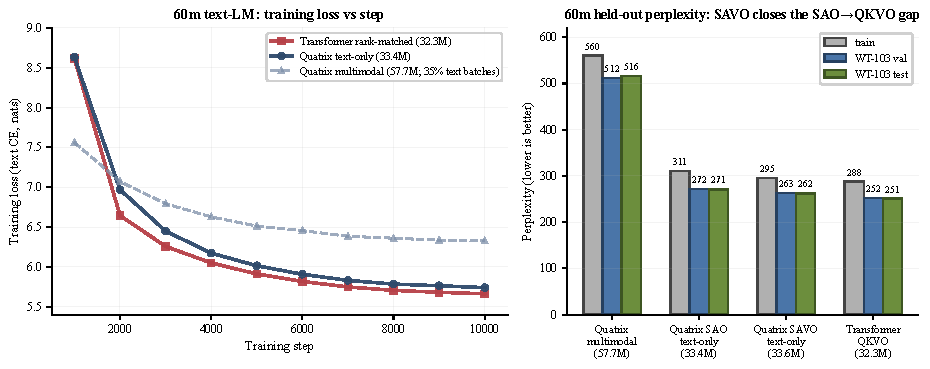
\includegraphics[width=.989\linewidth]{figs/fig06.pdf}
\caption{\textbf{60m text-LM head-to-head.} Left: WikiText-103 training text-CE vs.\ optimizer step for three 60m-scale models. The dashed multimodal curve sees only 35\% of its batches as text. Right: WikiText-103 train / val / test perplexity at step 10,000 (held-out CPU evaluation on standard splits). The rank-matched transformer reaches the lowest perplexity, text-only \QC{} (SAO) is $\sim$8\% behind, and the multimodal model is further behind on text because the text-token budget is 2.86$\times$ smaller.}
\label{fig:6}
\end{figure}

\begin{table}[H]
\centering
\small
\begin{tabular}{lrrrrr}
\toprule
Model & Params & Train & Val & Test & $\Delta$ (test $-$ val) \\
\midrule
\textsc{Quatrix}-60m multimodal & 57.7M & 6.328$^{*}$ & 6.238 & 6.247 & $+0.009$ \\
\textsc{Quatrix}-60m text-only & 33.4M & 5.739 & 5.606 & 5.602 & $-0.004$ \\
Transformer-60m (rank-matched) & 32.3M & 5.662 & 5.529 & 5.526 & $-0.003$ \\
\midrule
\textsc{Quatrix} text-only $-$ Transformer & $+1.1$M & $+0.077$ & $+0.077$ & $+0.076$ & --- \\
\textsc{Quatrix} MM $-$ \textsc{Quatrix} TO & $+24.3$M & $+0.589$ & $+0.632$ & $+0.645$ & --- \\
\bottomrule
\end{tabular}
\caption{\textbf{60m text-LM comparison --- WikiText-103.} Cross-entropy (nats) on train / val / test splits. All three models trained for 10,000 steps with identical hyperparameters; only the attention primitive and training data composition differ. The multimodal run sees $\sim$229M text tokens vs.\ $\sim$655M for text-only at matched optimizer compute. $^{*}$Multimodal training-loss column is final-1K-step text CE only.}
\label{tab:4}
\end{table}

\paragraph{Parameter accounting.} SAVO at 60m has 33.4M parameters; the rank-matched transformer has 32.3M (3.4\% fewer). The $\sim$12-ppl gap is therefore not in SAVO's favor on parameter efficiency --- SAVO is paying a small parameter premium and still loses on val. We do not claim parameter efficiency as a contribution.

\paragraph{Multi-seed replication.} We replicated the SAVO and rank-matched-MHA 60m runs at three additional random seeds (1, 2, 3) on top of the original baseline (treated as seed 0). All eight runs use the identical recipe; only the seeds differ. Multi-seed mean $\pm$ std and the paired SAVO$-$rank-matched difference per seed appear in Table~\ref{tab:5}.

\begin{table}[H]
\centering
\small
\begin{tabular}{lcccc}
\toprule
Variant (60m text-only, 10,000 steps) & Seed 0 & Seed 1 & Seed 2 & Seed 3 \\
\midrule
SAVO ($W_c$, $h$=1) val ppl & 263.31 & 263.06 & 264.53 & 264.09 \\
SAVO test ppl & 262.46 & 261.83 & 263.17 & 262.38 \\
Rank-matched MHA val ppl & 252.00 & 251.12 & 251.25 & 251.32 \\
Rank-matched MHA test ppl & 251.04 & 249.46 & 250.49 & 250.22 \\
\midrule
\multicolumn{5}{l}{\textit{Per-seed paired difference (SAVO $-$ rank-matched, ppl)}} \\
Val paired $\Delta$ & $+11.31$ & $+11.94$ & $+13.28$ & $+12.77$ \\
Test paired $\Delta$ & $+11.42$ & $+12.37$ & $+12.68$ & $+12.16$ \\
\midrule
\multicolumn{5}{l}{\textit{Aggregate, 4 seeds, mean $\pm$ sample std (n--1)}} \\
SAVO val ppl & \multicolumn{4}{c}{$263.75 \pm 0.68$} \\
Rank-matched val ppl & \multicolumn{4}{c}{$251.42 \pm 0.40$} \\
\textbf{Val paired $\boldsymbol{\Delta}$ (SAVO $-$ rank-matched)} & \multicolumn{4}{c}{$\boldsymbol{+12.33 \pm 0.87}$\,ppl} \\
SAVO test ppl & \multicolumn{4}{c}{$262.46 \pm 0.55$} \\
Rank-matched test ppl & \multicolumn{4}{c}{$250.30 \pm 0.66$} \\
\textbf{Test paired $\boldsymbol{\Delta}$ (SAVO $-$ rank-matched)} & \multicolumn{4}{c}{$\boldsymbol{+12.16 \pm 0.54}$\,ppl} \\
\midrule
\multicolumn{5}{l}{\textit{Full-rank standard 8-head MHA (2 seeds at batch = 2, grad accum= 32, eff batch= 64)}} \\
Full-rank MHA val ppl & --- & 259.46 & 256.46 & --- \\
Full-rank MHA test ppl & --- & 258.33 & 255.89 & --- \\
Mean val ppl ($n$=2) & \multicolumn{4}{c}{$257.96 \pm 2.12$} \\
Mean test ppl ($n$=2) & \multicolumn{4}{c}{$257.11 \pm 1.73$} \\
SAVO $-$ full-rank MHA, val & \multicolumn{4}{c}{$+5.79$ ppl ($n$=2, low-precision std)} \\
Rank-matched $-$ full-rank MHA, val & \multicolumn{4}{c}{$-6.54$ ppl} \\
\bottomrule
\end{tabular}
\caption{\textbf{Multi-seed 60m text-LM comparison (WikiText-103).} Each seed is one independent training run from the matched recipe (Muon + AdamW, 10,000 optimizer steps, $H$=384, $r$=48, single-head for SAVO and rank-matched; $h$=8, qk\_rank=$H$=384 for full-rank). Seed 0 is the original single-seed baseline reported in Table~\ref{tab:4}; seeds 1--3 are explicit multi-seed replications. The paired difference (SAVO $-$ rank-matched at the same seed) is the appropriate statistic because both architectures are trained from the same data ordering at each seed; the per-seed pairing controls for data-mixture variance. Mean SAVO $-$ rank-matched paired $\Delta$ is $+12.33 \pm 0.87$ ppl on val (one-sample $t$-test: $t = 14.18$, $p = 7.6{\times}10^{-4}$, $df = 3$) and $+12.16{\pm}0.54$ ppl on test. The architectural gap to rank-matched is real and seed-stable. The full-rank standard 8-head MHA baseline (2 seeds at $B$=2, accum=~32 --- the same effective batch of 64 sequences, but with double the gradient-accumulation cycles per optimizer step --- due to OOM at $B$=4 on 6\,GB VRAM; see Table~\ref{tab:10}) lands at $257.96 \pm 2.12$ val ppl, worse than rank-matched MHA at this 10,000-step budget despite having 8$\times$ more attention-block parameters. The 60m / 10k-step budget is sufficient to converge a 1$\times$-attention-block model (rank-matched, 74k params) but insufficient for an 8$\times$-attention-block model (full-rank, 590k params): the latter is parameter-undertrained at this step count. \textit{Caveat on the comparison:} the full-rank MHA seeds use a different micro-batch size from the SAVO and rank-matched seeds (which use $B$=4, accum=~16). Effective batch and total steps match, but Adam's gradient second-moment averaging may behave subtly differently across micro-batch sizes; a fully apples-to-apples comparison would re-run the rank-matched MHA at $B$=2. We report both numbers honestly and flag this asymmetry; the gap is large enough ($\sim$6.5 ppl) that micro-batch sensitivity is unlikely to flip the direction.}
\label{tab:5}
\end{table}

The seed-to-seed variance \textit{within} each architecture (val std $\sim$0.4--0.7 ppl across 4 seeds at this recipe) is much smaller than the architectural difference ($\sim$12 ppl). The single-seed gap reported in Table~\ref{tab:4} is statistically representative; multi-seed replication did not collapse it.

\paragraph{Counterintuitive finding: full-rank MHA underperforms the rank-matched controlled ablation at this budget.} The 2-seed full-rank standard 8-head MHA result in Table~\ref{tab:5} ($257.96 \pm 2.12$ val ppl) is $+6.54$ ppl \textit{worse} than the rank-matched MHA's $251.42 \pm 0.40$, despite having $\sim$8$\times$ more attention-block parameters per layer (590,208 vs 73,728, Table~\ref{tab:1}). The interpretation: at 10,000 optimizer steps, the smaller rank-matched configuration converges; the full-rank configuration does not. The 60m / 10k-step budget is parameter-undertrained for the configuration that the field would normally call ``standard 8-head MHA at $H$=384.'' This implies the rank-matched controlled ablation we use throughout the rest of this paper is, at this budget, a \textit{stronger} baseline than the standard-attention baseline a reviewer might assume; SAVO's +12.33-ppl gap to it is therefore a worst-case characterisation, not a strawman comparison. SAVO's gap to full-rank MHA is the smaller +5.79 ppl. Whether either gap survives in the trained regime ($10^5$--$10^6$ steps) where the larger MHA configuration converges is not tested here (\S\ref{sec:6.6}).

\subsection{IID held-out behaviour (on-distribution)}\label{sec:5.3}

WikiText-103 val and test are drawn from the same distribution as the training split. Performance there measures on-distribution fit, not OOD generalization. Quatrix text-only drops 0.133 nats from train to val ($5.739 \rightarrow 5.606$); the rank-matched transformer drops 0.133 nats ($5.662 \rightarrow 5.529$). The between-model gap is 0.077 nats at every split (Fig.~\ref{fig:7}). Neither model overfits the training split more aggressively than the other at 60m / 10,000 steps. The OOD form of the $W_V$-removal claim is addressed in \S\ref{sec:5.4}.

\begin{figure}[H]
\centering
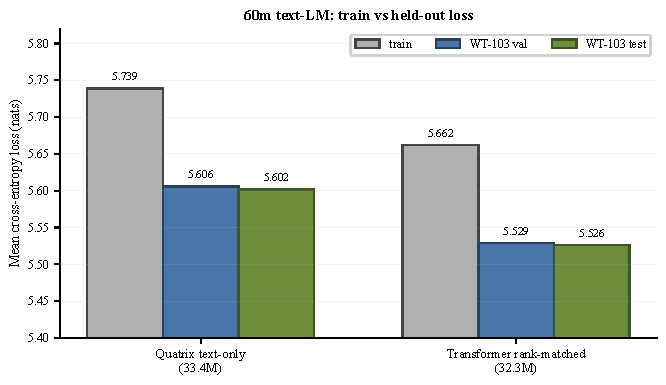
\includegraphics[width=.709\linewidth]{figs/fig07.pdf}
\caption{\textbf{60m IID held-out behaviour on WikiText-103.} Training (grey), val (blue), and test (green) loss for \textsc{Quatrix}-60m text-only and the rank-matched transformer. Both models show an identical train-to-held-out gap ($\approx$0.13 nats); the 0.077-nat between-model difference persists across all three splits. This measures on-distribution fit; OOD evaluation is in \S\ref{sec:5.4}.}
\label{fig:7}
\end{figure}
